\documentclass[border=12pt]{standalone}
\def\pgfsysdriver{pgfsys-dvisvgm.def}
\usepackage[dvisvgm]{xcolor}
\usepackage{xeCJK}
\setCJKmainfont{HaranoAjiGothic-Regular.otf}[BoldFont=HaranoAjiGothic-Bold.otf]
\setCJKsansfont{HaranoAjiGothic-Regular.otf}[BoldFont=HaranoAjiGothic-Bold.otf]
\usepackage{amsmath,amssymb,tikz,lmodern}
\usetikzlibrary{arrows.meta,positioning,calc,fit,backgrounds}
\renewcommand{\familydefault}{\sfdefault}
\definecolor{ink}{HTML}{25322F}
\definecolor{green}{HTML}{246657}
\definecolor{tint}{HTML}{EEF4F0}
\definecolor{soft}{HTML}{C6D2CC}
\definecolor{muted}{HTML}{52615B}
\newif\ifJapanese
\newcommand{\Tx}[2]{\ifJapanese #1\else #2\fi}
\newcommand{\Eff}{\overline{\operatorname{Eff}}}
\newcommand{\heading}[3]{{\color{green}\bfseries #1\quad\Tx{#2}{#3}}\\[5pt]}
% A white rectangle makes the complete citation label clickable, including spaces.
\newcommand{\refurl}[2]{\special{dvisvgm:raw <a xlink:href="#1" target="_blank" rel="noopener noreferrer">}{\setlength{\fboxsep}{0pt}\colorbox{white}{\color{green}\underline{\strut #2}}}\special{dvisvgm:raw </a>}}
\tikzset{
 card/.style={draw=soft,fill=white,rounded corners=2pt,align=left,text=ink,font=\fontsize{10.5}{14}\selectfont,inner xsep=12pt,inner ysep=10pt,text width=14.4cm},
 half/.style={card,text width=6.45cm,minimum height=2.05cm},
 result/.style={card,draw=green,fill=tint,line width=.9pt},
 reason/.style={align=left,text=muted,font=\fontsize{9}{12}\selectfont,inner sep=0pt,text width=12.7cm},
 branchreason/.style={reason,text width=5.95cm},
 edge/.style={-{Stealth[length=2.4mm]},draw=green,line width=1pt},
 wire/.style={draw=green,line width=1pt},
}
% Keep the arrow in a dedicated left gutter; explanations never cover it.
\newcommand{\flow}[3]{
 \coordinate (#2-from) at ($(#1.south)+(-6.9,0)$);
 \coordinate (#2-to) at ($(#2.north)+(-6.9,0)$);
 \draw[edge] (#2-from)--(#2-to);
 \node[reason,anchor=west] (#2-reason) at ($(#2-from)!.5!(#2-to)+(.55,0)$) {#3};
}

\newcommand{\Cite}[2]{\refurl{#1}{#2}}

\Japanesetrue
\begin{document}
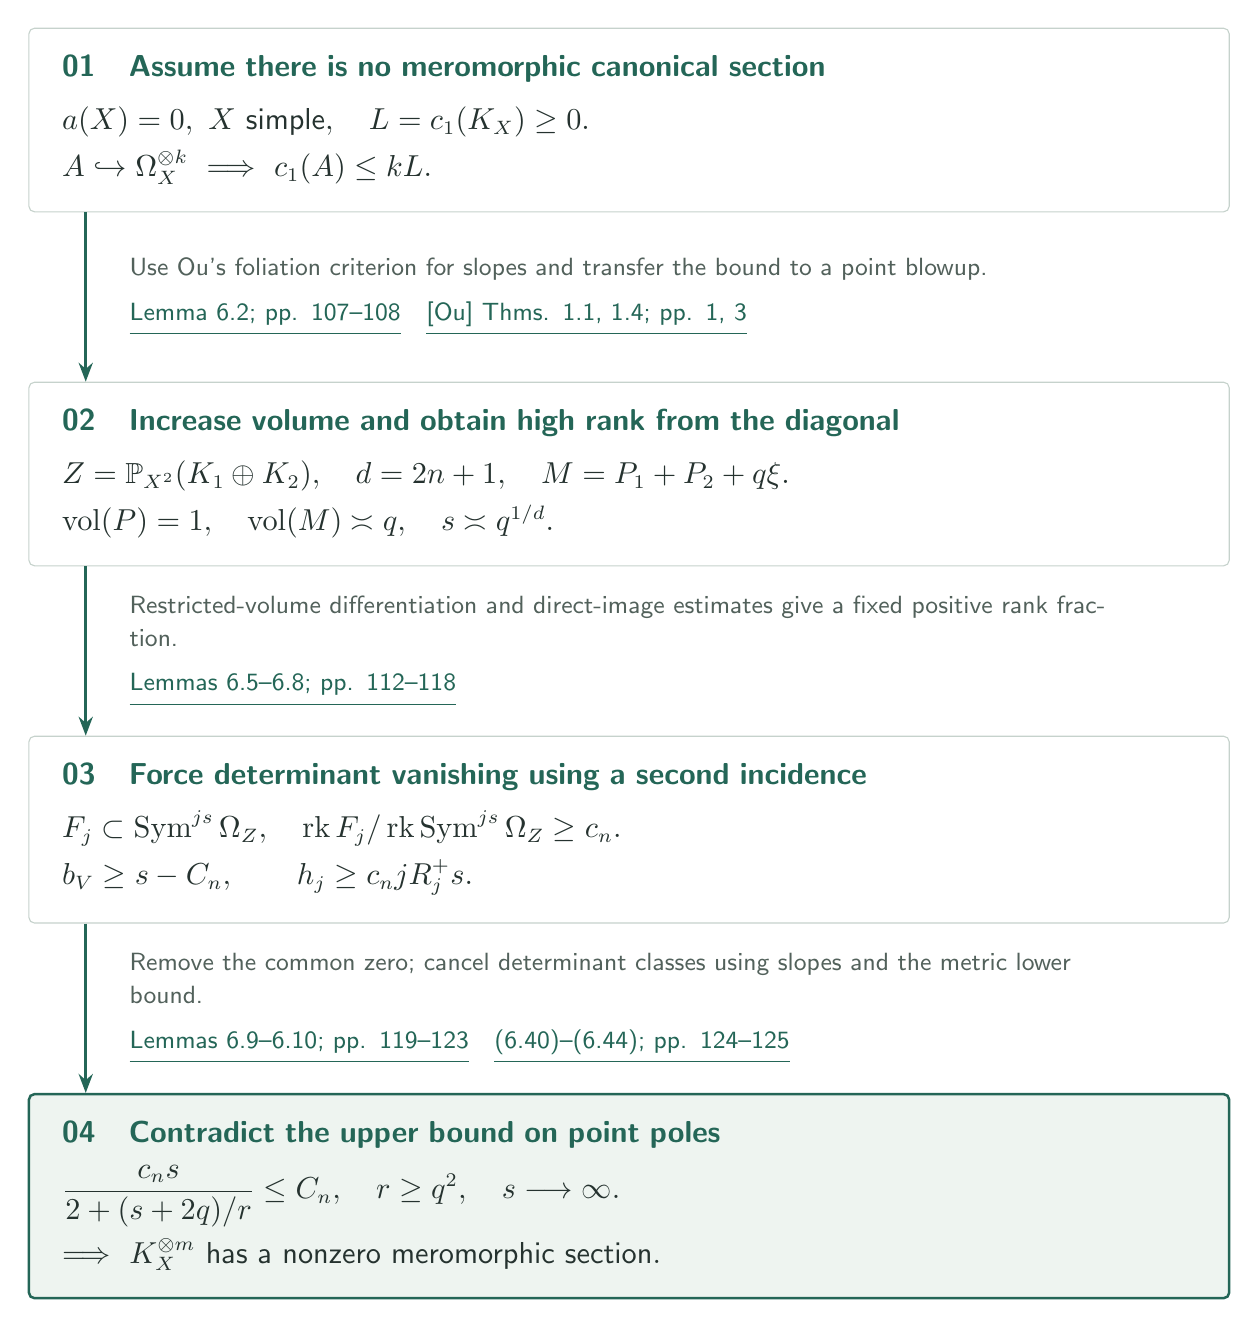
\begin{tikzpicture}
\node[card] (n0) {\heading{01}{有理型標準切断がないと仮定する}{Assume there is no meromorphic canonical section}$a(X)=0,\ X\text{ simple},\quad L=c_1(K_X)\ge0.$\\[3pt] $A\hookrightarrow\Omega_X^{\otimes k}\ \Longrightarrow\ c_1(A)\le kL.$};
\node[card,below=2.15cm of n0] (n1) {\heading{02}{体積を増やし、対角線で高rankを作る}{Increase volume and obtain high rank from the diagonal}$Z=\mathbb P_{X^2}(K_1\oplus K_2),\quad d=2n+1,\quad M=P_1+P_2+q\xi.$\\[3pt] $\operatorname{vol}(P)=1,\quad\operatorname{vol}(M)\asymp q,\quad s\asymp q^{1/d}.$};
\flow{n0}{n1}{\Tx{Ouの葉層判定でslopeを抑え、点のblowupへ運ぶ。}{Use Ou’s foliation criterion for slopes and transfer the bound to a point blowup.}\\[4pt]\Cite{https://github.com/openai/math/blob/adc7f1241b42e322a6451854ab7e4b4c146bf78a/preprints/Log-abundance-for-compact-Kahler-spaces-under-logarithmic-Iitaka-subadditivity-October-4-2026/main.pdf}{Lemma 6.2; pp. 107--108}\quad \Cite{https://arxiv.org/pdf/2501.18088v1}{[Ou] Thms. 1.1, 1.4; pp. 1, 3}}
\node[card,below=2.15cm of n1] (n2) {\heading{03}{第二のincidenceで行列式の消滅を強制}{Force determinant vanishing using a second incidence}$F_j\subset\operatorname{Sym}^{js}\Omega_Z,\quad \operatorname{rk}F_j/\operatorname{rk}\operatorname{Sym}^{js}\Omega_Z\ge c_n.$\\[3pt] $b_V\ge s-C_n,\qquad h_j\ge c_n jR_j^+s.$};
\flow{n1}{n2}{\Tx{制限体積の微分とdirect-image評価から固定正割合のrankを得る。}{Restricted-volume differentiation and direct-image estimates give a fixed positive rank fraction.}\\[4pt]\Cite{https://github.com/openai/math/blob/adc7f1241b42e322a6451854ab7e4b4c146bf78a/preprints/Log-abundance-for-compact-Kahler-spaces-under-logarithmic-Iitaka-subadditivity-October-4-2026/main.pdf}{Lemmas 6.5--6.8; pp. 112--118}}
\node[result,below=2.15cm of n2] (n3) {\heading{04}{点の極の上界と矛盾させる}{Contradict the upper bound on point poles}$\displaystyle \frac{c_ns}{2+(s+2q)/r}\le C_n,\quad r\ge q^2,\quad s\longrightarrow\infty.$\\[3pt] $\Longrightarrow\ K_X^{\otimes m}\Tx{\text{ に非零有理型切断が存在}}{\text{ has a nonzero meromorphic section}}.$};
\flow{n2}{n3}{\Tx{共通零因子を除き、slope評価とmetricの下界で行列式の類を相殺。}{Remove the common zero; cancel determinant classes using slopes and the metric lower bound.}\\[4pt]\Cite{https://github.com/openai/math/blob/adc7f1241b42e322a6451854ab7e4b4c146bf78a/preprints/Log-abundance-for-compact-Kahler-spaces-under-logarithmic-Iitaka-subadditivity-October-4-2026/main.pdf}{Lemmas 6.9--6.10; pp. 119--123}\quad \Cite{https://github.com/openai/math/blob/adc7f1241b42e322a6451854ab7e4b4c146bf78a/preprints/Log-abundance-for-compact-Kahler-spaces-under-logarithmic-Iitaka-subadditivity-October-4-2026/main.pdf}{(6.40)--(6.44); pp. 124--125}}
\end{tikzpicture}

\end{document}
